% Part 6: Multi-Tier Agent Architecture
% A Comprehensive Guide to Hierarchical Agentic Systems
% Beamer Presentation with UofSC Color Scheme

\documentclass[aspectratio=169,11pt]{beamer}

% ============================================
% THEME AND COLOR CONFIGURATION
% ============================================
\usetheme{Madrid}
\usecolortheme{default}

% UofSC Color Definitions
\definecolor{UofSCGarnet}{HTML}{73000a}
\definecolor{UofSCBlack}{HTML}{000000}
\definecolor{UofSCWhite}{HTML}{ffffff}
\definecolor{UofSCRose}{HTML}{CC2E40}
\definecolor{UofSCAtlantic}{HTML}{466A9F}
\definecolor{UofSCCongaree}{HTML}{1F414D}
\definecolor{UofSCHorseshoe}{HTML}{65780B}
\definecolor{UofSCGrass}{HTML}{CED318}
\definecolor{UofSCHoneycomb}{HTML}{A49137}
\definecolor{UofSC90Black}{HTML}{363636}
\definecolor{UofSC70Black}{HTML}{5C5C5C}
\definecolor{UofSC50Black}{HTML}{A2A2A2}
\definecolor{UofSCWarmGrey}{HTML}{676156}
\definecolor{UofSCSandstorm}{HTML}{FFF2E3}
\definecolor{UofSCDarkGarnet}{HTML}{570008}
\definecolor{UofSCAzalea}{HTML}{844247}

% Apply UofSC colors to Beamer theme
\setbeamercolor{palette primary}{bg=UofSCGarnet,fg=UofSCWhite}
\setbeamercolor{palette secondary}{bg=UofSCCongaree,fg=UofSCWhite}
\setbeamercolor{palette tertiary}{bg=UofSCAtlantic,fg=UofSCWhite}
\setbeamercolor{palette quaternary}{bg=UofSCBlack,fg=UofSCWhite}
\setbeamercolor{structure}{fg=UofSCGarnet}
\setbeamercolor{section in toc}{fg=UofSCGarnet}
\setbeamercolor{subsection in toc}{fg=UofSCCongaree}
\setbeamercolor{title}{fg=UofSCWhite,bg=UofSCGarnet}
\setbeamercolor{frametitle}{fg=UofSCWhite,bg=UofSCGarnet}
\setbeamercolor{block title}{bg=UofSCGarnet,fg=UofSCWhite}
\setbeamercolor{block body}{bg=UofSCSandstorm,fg=UofSCBlack}
\setbeamercolor{block title alerted}{bg=UofSCRose,fg=UofSCWhite}
\setbeamercolor{block body alerted}{bg=UofSCSandstorm,fg=UofSCBlack}
\setbeamercolor{block title example}{bg=UofSCAtlantic,fg=UofSCWhite}
\setbeamercolor{block body example}{bg=UofSCSandstorm,fg=UofSCBlack}
\setbeamercolor{itemize item}{fg=UofSCGarnet}
\setbeamercolor{itemize subitem}{fg=UofSCCongaree}
\setbeamercolor{enumerate item}{fg=UofSCGarnet}
\setbeamercolor{enumerate subitem}{fg=UofSCCongaree}
\setbeamercolor{footnote}{fg=UofSC70Black}
\setbeamercolor{caption name}{fg=UofSCGarnet}

% Remove rounded corners (sharp edges per style guide)
\setbeamertemplate{blocks}[default]
\setbeamertemplate{title page}[default][colsep=-4bp]
\setbeamertemplate{itemize items}[square]
\setbeamertemplate{enumerate items}[default]

% Navigation symbols
\setbeamertemplate{navigation symbols}{}

% Footline with page numbers
\setbeamertemplate{footline}{
  \leavevmode%
  \hbox{%
  \begin{beamercolorbox}[wd=.333333\paperwidth,ht=2.25ex,dp=1ex,center]{author in head/foot}%
    \usebeamerfont{author in head/foot}\insertshortauthor
  \end{beamercolorbox}%
  \begin{beamercolorbox}[wd=.333333\paperwidth,ht=2.25ex,dp=1ex,center]{title in head/foot}%
    \usebeamerfont{title in head/foot}\insertshorttitle
  \end{beamercolorbox}%
  \begin{beamercolorbox}[wd=.333333\paperwidth,ht=2.25ex,dp=1ex,right]{date in head/foot}%
    \usebeamerfont{date in head/foot}\insertshortdate{}\hspace*{2em}
    \insertframenumber{} / \inserttotalframenumber\hspace*{2ex}
  \end{beamercolorbox}}%
  \vskip0pt%
}

% ============================================
% PACKAGES
% ============================================
\usepackage[utf8]{inputenc}
\usepackage[T1]{fontenc}
\usepackage{lmodern}
\usepackage{amsmath,amssymb,amsfonts}
\usepackage{graphicx}
\usepackage{tikz}
\usetikzlibrary{shapes,arrows.meta,positioning,calc,fit,backgrounds,chains,decorations.pathreplacing}
\usepackage{listings}
\usepackage{booktabs}
\usepackage{array}
\usepackage{hyperref}
\usepackage{xcolor}
\usepackage{multicol}

% TikZ styles for diagrams (sharp corners, no rounded edges)
\tikzset{
    % Base node style
    basenode/.style={
        draw=UofSCBlack,
        fill=UofSCWhite,
        line width=0.8pt,
        minimum height=0.8cm,
        minimum width=2cm,
        align=center,
        font=\small
    },
    % Strategy layer style
    strategynode/.style={
        basenode,
        fill=UofSCGarnet,
        text=UofSCWhite,
        minimum height=1cm,
        minimum width=4cm
    },
    % Planning layer style
    planningnode/.style={
        basenode,
        fill=UofSCAtlantic,
        text=UofSCWhite,
        minimum height=0.9cm,
        minimum width=3.5cm
    },
    % Execution layer style
    execnode/.style={
        basenode,
        fill=UofSCCongaree,
        text=UofSCWhite,
        minimum height=0.8cm,
        minimum width=2.5cm
    },
    % Generic box
    genericbox/.style={
        basenode,
        minimum width=2.8cm
    },
    % Arrow styles (straight lines only)
    myarrow/.style={
        ->,
        >=Stealth,
        line width=0.8pt,
        draw=UofSCBlack
    },
    % Bidirectional arrow
    biarrow/.style={
        <->,
        >=Stealth,
        line width=0.8pt,
        draw=UofSCBlack
    },
    % Phase box style
    phasebox/.style={
        basenode,
        minimum width=3.5cm,
        minimum height=1.2cm,
        font=\small\bfseries
    },
    % Small box
    smallbox/.style={
        basenode,
        minimum width=1.5cm,
        minimum height=0.6cm,
        font=\scriptsize
    },
    % Leader node
    leadernode/.style={
        basenode,
        fill=UofSCGarnet,
        text=UofSCWhite,
        minimum width=3cm,
        minimum height=1cm
    },
    % Worker node
    workernode/.style={
        basenode,
        fill=UofSC70Black,
        text=UofSCWhite,
        minimum width=1.2cm,
        minimum height=0.7cm,
        font=\scriptsize
    }
}

% Listings configuration
\lstset{
    basicstyle=\ttfamily\scriptsize,
    keywordstyle=\color{UofSCGarnet}\bfseries,
    commentstyle=\color{UofSC70Black}\itshape,
    stringstyle=\color{UofSCAtlantic},
    numberstyle=\tiny\color{UofSC50Black},
    numbers=left,
    numbersep=5pt,
    frame=single,
    framerule=0.5pt,
    rulecolor=\color{UofSC50Black},
    backgroundcolor=\color{UofSCSandstorm},
    breaklines=true,
    breakatwhitespace=true,
    tabsize=2,
    showstringspaces=false,
    captionpos=b
}

% Python language for listings
\lstdefinelanguage{Python}{
    keywords={def,class,if,elif,else,for,while,return,import,from,as,try,except,with,lambda,True,False,None,and,or,not,in,is},
    morecomment=[l]{\#},
    morestring=[b]",
    morestring=[b]',
    sensitive=true
}

% ============================================
% DOCUMENT METADATA
% ============================================
\title[Part 6: Multi-Tier Architecture]{Part 6: Multi-Tier Agent Architecture}
\subtitle{Building Hierarchical Systems with Agentic Coding Tools}
\author{Advanced Agentic Coding Tools Course}
\institute{University of South Carolina}
\date{\today}

% ============================================
% DOCUMENT BEGIN
% ============================================
\begin{document}

% Title slide
\begin{frame}[plain]
    \titlepage
\end{frame}

% Table of Contents
\begin{frame}{Outline}
    \tableofcontents
\end{frame}

% ============================================
% SECTION 1: Beyond Two Layers
% ============================================
\section{Beyond Two Layers}

\begin{frame}{Why Stop at Two Layers?}
    \begin{columns}[T]
        \begin{column}{0.5\textwidth}
            \textbf{Two-Layer Limitation:}
            \begin{center}
            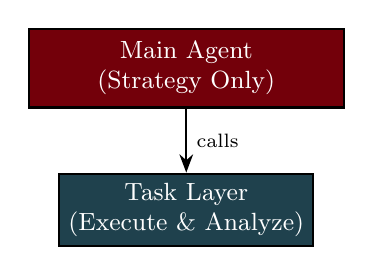
\begin{tikzpicture}[scale=0.9]
                \node[strategynode] (main) at (0,2) {Main Agent\\(Strategy Only)};
                \node[execnode] (task) at (0,0) {Task Layer\\(Execute \& Analyze)};
                \draw[myarrow] (main) -- node[right,font=\scriptsize]{calls} (task);
            \end{tikzpicture}
            \end{center}
        \end{column}
        \begin{column}{0.5\textwidth}
            \textbf{Issues:}
            \begin{itemize}
                \item All complexity forced into task execution
                \item Poor separation of concerns
                \item Limited nuanced decision handling
                \item No intermediate planning layer
                \item Difficult multi-domain management
            \end{itemize}
        \end{column}
    \end{columns}

    \vspace{0.5cm}
    \begin{block}{Key Insight}
        Real-world problems require multiple levels of abstraction that do not fit neatly into ``main agent'' and ``task.''
    \end{block}

    \note{
        Two-layer systems work for simpler problems but break down when:
        1. The problem domain requires multiple levels of abstraction
        2. Tasks themselves need decomposition
        3. Different specialists need to collaborate
        4. Cross-domain knowledge is required
    }
\end{frame}

\begin{frame}{Complex Problem Decomposition}
    \begin{center}
    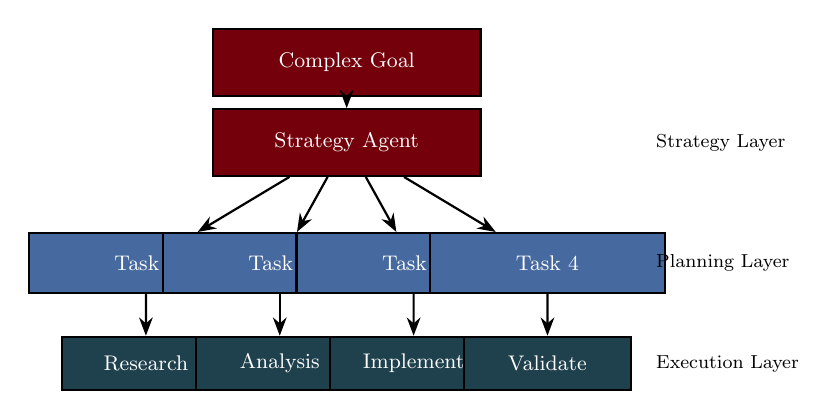
\begin{tikzpicture}[scale=0.85, transform shape]
        % Top level
        \node[strategynode] (goal) at (0,5) {Complex Goal};
        \node[strategynode] (strategy) at (0,3.8) {Strategy Agent};

        % Planning level
        \node[planningnode] (p1) at (-3,2) {Task 1};
        \node[planningnode] (p2) at (-1,2) {Task 2};
        \node[planningnode] (p3) at (1,2) {Task 3};
        \node[planningnode] (p4) at (3,2) {Task 4};

        % Execution level
        \node[execnode] (e1) at (-3,0.5) {Research};
        \node[execnode] (e2) at (-1,0.5) {Analysis};
        \node[execnode] (e3) at (1,0.5) {Implement};
        \node[execnode] (e4) at (3,0.5) {Validate};

        % Arrows
        \draw[myarrow] (goal) -- (strategy);
        \draw[myarrow] (strategy) -- (p1);
        \draw[myarrow] (strategy) -- (p2);
        \draw[myarrow] (strategy) -- (p3);
        \draw[myarrow] (strategy) -- (p4);

        \draw[myarrow] (p1) -- (e1);
        \draw[myarrow] (p2) -- (e2);
        \draw[myarrow] (p3) -- (e3);
        \draw[myarrow] (p4) -- (e4);

        % Labels
        \node[font=\footnotesize,right] at (4.5,3.8) {Strategy Layer};
        \node[font=\footnotesize,right] at (4.5,2) {Planning Layer};
        \node[font=\footnotesize,right] at (4.5,0.5) {Execution Layer};
    \end{tikzpicture}
    \end{center}

    \vspace{0.3cm}
    \textbf{Multi-Level Decomposition Benefits:}
    \begin{itemize}
        \item Strategy: High-level reasoning about what to do
        \item Planning: How to break this into manageable pieces
        \item Execution: Specific actions to accomplish each piece
    \end{itemize}
\end{frame}

\begin{frame}{Scaling Through Delegation}
    \begin{columns}[T]
        \begin{column}{0.45\textwidth}
            \textbf{Linear (2-layer):}
            \begin{itemize}
                \item Size of work $\rightarrow$ Complexity of main agent
                \item One agent handles everything
                \item Problem: Cognitive overload
            \end{itemize}

            \vspace{0.5cm}
            \textbf{Hierarchical (3+ layer):}
            \begin{itemize}
                \item Size of work $\rightarrow$ More agents
                \item Distributed problem solving
                \item Parallelization \& specialization
            \end{itemize}
        \end{column}
        \begin{column}{0.55\textwidth}
            \begin{center}
            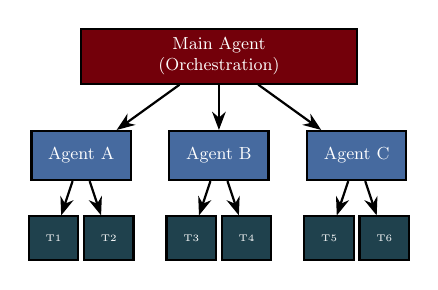
\begin{tikzpicture}[scale=0.7, transform shape]
                % Main agent
                \node[strategynode,minimum width=5cm] (main) at (0,4) {Main Agent\\(Orchestration)};

                % Level 2
                \node[planningnode,minimum width=1.8cm] (a) at (-2.5,2.2) {Agent A};
                \node[planningnode,minimum width=1.8cm] (b) at (0,2.2) {Agent B};
                \node[planningnode,minimum width=1.8cm] (c) at (2.5,2.2) {Agent C};

                % Level 3
                \node[execnode,minimum width=0.9cm,font=\tiny] (t1) at (-3,0.7) {T1};
                \node[execnode,minimum width=0.9cm,font=\tiny] (t2) at (-2,0.7) {T2};
                \node[execnode,minimum width=0.9cm,font=\tiny] (t3) at (-0.5,0.7) {T3};
                \node[execnode,minimum width=0.9cm,font=\tiny] (t4) at (0.5,0.7) {T4};
                \node[execnode,minimum width=0.9cm,font=\tiny] (t5) at (2,0.7) {T5};
                \node[execnode,minimum width=0.9cm,font=\tiny] (t6) at (3,0.7) {T6};

                % Arrows
                \draw[myarrow] (main) -- (a);
                \draw[myarrow] (main) -- (b);
                \draw[myarrow] (main) -- (c);
                \draw[myarrow] (a) -- (t1);
                \draw[myarrow] (a) -- (t2);
                \draw[myarrow] (b) -- (t3);
                \draw[myarrow] (b) -- (t4);
                \draw[myarrow] (c) -- (t5);
                \draw[myarrow] (c) -- (t6);
            \end{tikzpicture}
            \end{center}
        \end{column}
    \end{columns}

    \vspace{0.3cm}
    \begin{alertblock}{Parallelization Benefits}
        Multiple tasks execute simultaneously, better resource utilization, faster completion, specialized expertise at each level.
    \end{alertblock}
\end{frame}

\begin{frame}{When to Use Multi-Tier Systems}
    \begin{columns}[T]
        \begin{column}{0.5\textwidth}
            \textbf{Multi-Tier Systems Excel At:}
            \begin{itemize}
                \item[\checkmark] Large codebase modifications
                \item[\checkmark] Research and analysis tasks
                \item[\checkmark] Multi-phase projects
                \item[\checkmark] Cross-domain problems
                \item[\checkmark] Multiple perspectives needed
                \item[\checkmark] High availability requirements
            \end{itemize}
        \end{column}
        \begin{column}{0.5\textwidth}
            \textbf{Common Scenarios:}
            \begin{enumerate}
                \item \textbf{Software Engineering:}\\Architecture $\rightarrow$ Design $\rightarrow$ Implementation
                \item \textbf{Research:}\\Lit review $\rightarrow$ Analysis $\rightarrow$ Writing
                \item \textbf{Data Processing:}\\Validate $\rightarrow$ Transform $\rightarrow$ Report
                \item \textbf{DevOps:}\\Plan $\rightarrow$ Configure $\rightarrow$ Deploy
            \end{enumerate}
        \end{column}
    \end{columns}

    \vspace{0.3cm}
    \begin{block}{Decision Criteria}
        Use multi-tier when: problem naturally decomposes into levels, different expertise needed at stages, task size is large, parallelization is beneficial, results need intelligent aggregation.
    \end{block}
\end{frame}

% ============================================
% SECTION 2: Three-Tier Framework
% ============================================
\section{Three-Tier Framework}

\begin{frame}{The Three-Tier Foundation}
    \begin{center}
    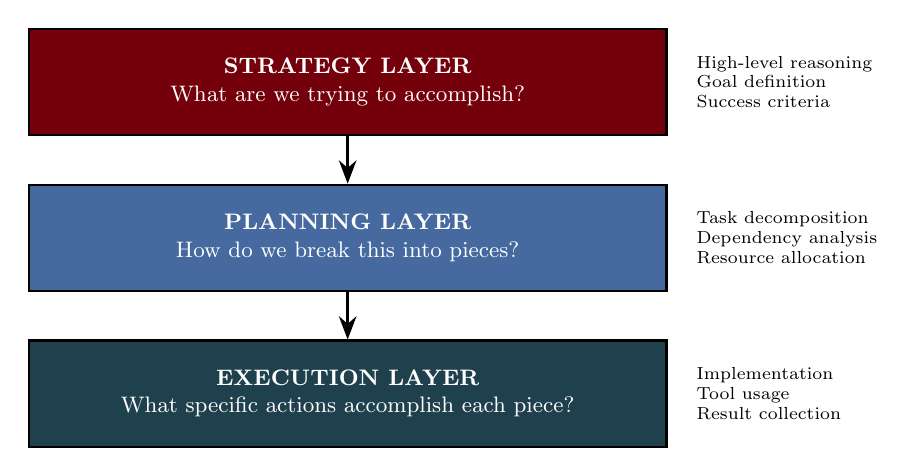
\begin{tikzpicture}[scale=0.9, transform shape]
        % Strategy Layer
        \node[strategynode, minimum width=9cm, minimum height=1.5cm] (strategy) at (0,5) {
            \textbf{STRATEGY LAYER}\\
            What are we trying to accomplish?
        };
        \node[font=\scriptsize, align=left, right] at (4.8,5) {
            High-level reasoning\\
            Goal definition\\
            Success criteria
        };

        % Planning Layer
        \node[planningnode, minimum width=9cm, minimum height=1.5cm] (planning) at (0,2.8) {
            \textbf{PLANNING LAYER}\\
            How do we break this into pieces?
        };
        \node[font=\scriptsize, align=left, right] at (4.8,2.8) {
            Task decomposition\\
            Dependency analysis\\
            Resource allocation
        };

        % Execution Layer
        \node[execnode, minimum width=9cm, minimum height=1.5cm] (exec) at (0,0.6) {
            \textbf{EXECUTION LAYER}\\
            What specific actions accomplish each piece?
        };
        \node[font=\scriptsize, align=left, right] at (4.8,0.6) {
            Implementation\\
            Tool usage\\
            Result collection
        };

        % Arrows
        \draw[myarrow, line width=1.2pt] (strategy) -- (planning);
        \draw[myarrow, line width=1.2pt] (planning) -- (exec);
    \end{tikzpicture}
    \end{center}

    \vspace{0.3cm}
    \begin{columns}[T]
        \begin{column}{0.5\textwidth}
            \textbf{Why Three Layers?}
            \begin{itemize}
                \item Beyond 3: diminishing returns, increased latency
                \item Less than 3: insufficient abstraction
                \item Three provides sweet spot for most problems
            \end{itemize}
        \end{column}
        \begin{column}{0.5\textwidth}
            \textbf{This mirrors:}
            \begin{itemize}
                \item Human problem-solving approaches
                \item OpenHands, AutoGPT architectures
                \item Claude Code internal structure
            \end{itemize}
        \end{column}
    \end{columns}
\end{frame}

\begin{frame}{Strategy Layer Deep Dive}
    \begin{columns}[T]
        \begin{column}{0.55\textwidth}
            \textbf{Strategy Layer Responsibilities:}
            \begin{itemize}
                \item Receive high-level goal
                \item Analyze problem domain
                \item Identify constraints
                \item Define success criteria
                \item Make major strategic decisions
                \item Decompose into major phases
                \item Output: Strategic Plan
            \end{itemize}

            \vspace{0.3cm}
            \textbf{Key Characteristics:}
            \begin{itemize}
                \item Highest-level abstraction
                \item Domain-specific reasoning
                \item Uses external knowledge
                \item Makes irreversible decisions
            \end{itemize}
        \end{column}
        \begin{column}{0.45\textwidth}
            \begin{exampleblock}{Example Input}
                ``Build a data pipeline to process customer transaction logs and generate weekly reports''
            \end{exampleblock}

            \vspace{0.2cm}
            \begin{block}{Processing Steps}
                \begin{enumerate}
                    \item Understand problem scope
                    \item Identify major phases
                    \item Determine key technologies
                    \item Define quality standards
                    \item Plan resource allocation
                \end{enumerate}
            \end{block}
        \end{column}
    \end{columns}
\end{frame}

\begin{frame}{Planning Layer Deep Dive}
    \textbf{Planning Layer Responsibilities:}
    \begin{itemize}
        \item Receive strategic plan
        \item Decompose into executable tasks
        \item Analyze dependencies
        \item Optimize execution order
        \item Allocate resources
    \end{itemize}

    \vspace{0.3cm}
    \begin{center}
    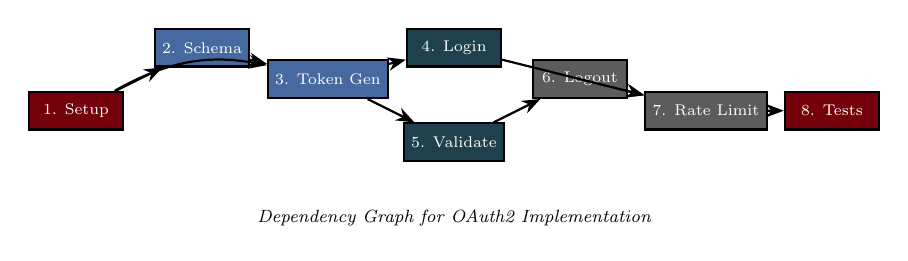
\begin{tikzpicture}[scale=0.8, transform shape]
        % Task nodes
        \node[smallbox, fill=UofSCGarnet, text=white] (t1) at (0,2) {1. Setup};
        \node[smallbox, fill=UofSCAtlantic, text=white] (t2) at (2,3) {2. Schema};
        \node[smallbox, fill=UofSCAtlantic, text=white] (t3) at (4,2.5) {3. Token Gen};
        \node[smallbox, fill=UofSCCongaree, text=white] (t4) at (6,3) {4. Login};
        \node[smallbox, fill=UofSCCongaree, text=white] (t5) at (6,1.5) {5. Validate};
        \node[smallbox, fill=UofSC70Black, text=white] (t6) at (8,2.5) {6. Logout};
        \node[smallbox, fill=UofSC70Black, text=white] (t7) at (10,2) {7. Rate Limit};
        \node[smallbox, fill=UofSCGarnet, text=white] (t8) at (12,2) {8. Tests};

        % Arrows showing dependencies
        \draw[myarrow] (t1) -- (t2);
        \draw[myarrow] (t1) to[bend left=20] (t3);
        \draw[myarrow] (t2) -- (t3);
        \draw[myarrow] (t3) -- (t4);
        \draw[myarrow] (t3) -- (t5);
        \draw[myarrow] (t5) -- (t6);
        \draw[myarrow] (t4) -- (t7);
        \draw[myarrow] (t6) -- (t7);
        \draw[myarrow] (t7) -- (t8);

        % Label
        \node[font=\footnotesize\itshape] at (6,0.3) {Dependency Graph for OAuth2 Implementation};
    \end{tikzpicture}
    \end{center}

    \textbf{Planning Strategies:} Topological sorting, Parallelization identification, Load balancing, Error recovery planning
\end{frame}

\begin{frame}{Execution Layer Deep Dive}
    \begin{columns}[T]
        \begin{column}{0.5\textwidth}
            \textbf{Execution Task Lifecycle:}
            \begin{center}
            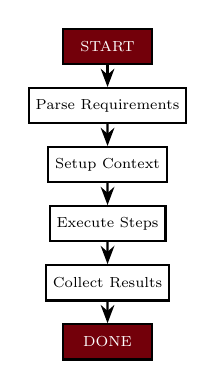
\begin{tikzpicture}[scale=0.75, transform shape]
                \node[smallbox, fill=UofSCGarnet, text=white] (start) at (0,5) {START};
                \node[smallbox] (parse) at (0,4) {Parse Requirements};
                \node[smallbox] (setup) at (0,3) {Setup Context};
                \node[smallbox] (exec) at (0,2) {Execute Steps};
                \node[smallbox] (collect) at (0,1) {Collect Results};
                \node[smallbox, fill=UofSCGarnet, text=white] (done) at (0,0) {DONE};

                \draw[myarrow] (start) -- (parse);
                \draw[myarrow] (parse) -- (setup);
                \draw[myarrow] (setup) -- (exec);
                \draw[myarrow] (exec) -- (collect);
                \draw[myarrow] (collect) -- (done);
            \end{tikzpicture}
            \end{center}
        \end{column}
        \begin{column}{0.5\textwidth}
            \textbf{Available Tools:}
            \begin{itemize}
                \item File operations (read, write, edit)
                \item Code execution (run tests, lint)
                \item Build systems
                \item Package managers
                \item Version control
                \item APIs and external services
            \end{itemize}

            \vspace{0.3cm}
            \textbf{Execution Patterns:}
            \begin{itemize}
                \item Deterministic when possible
                \item Retry logic for transient failures
                \item Progress reporting
                \item Resource cleanup
                \item Artifact collection
            \end{itemize}
        \end{column}
    \end{columns}
\end{frame}

\begin{frame}{Information Flow Between Layers}
    \begin{center}
    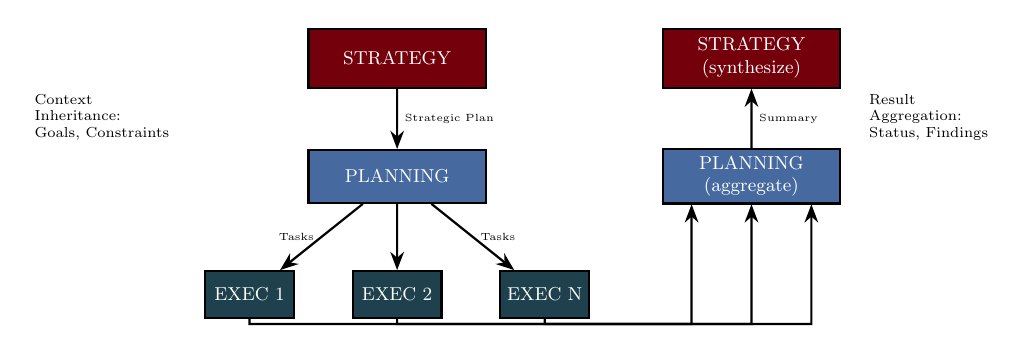
\begin{tikzpicture}[scale=0.75, transform shape]
        % Strategy
        \node[strategynode, minimum width=3cm] (s1) at (0,5) {STRATEGY};

        % Planning
        \node[planningnode, minimum width=3cm] (p1) at (0,3) {PLANNING};

        % Execution agents
        \node[execnode, minimum width=1.5cm] (e1) at (-2.5,1) {EXEC 1};
        \node[execnode, minimum width=1.5cm] (e2) at (0,1) {EXEC 2};
        \node[execnode, minimum width=1.5cm] (e3) at (2.5,1) {EXEC N};

        % Planning synthesis
        \node[planningnode, minimum width=3cm] (p2) at (6,3) {PLANNING\\(aggregate)};

        % Strategy synthesis
        \node[strategynode, minimum width=3cm] (s2) at (6,5) {STRATEGY\\(synthesize)};

        % Downward arrows
        \draw[myarrow] (s1) -- node[right,font=\tiny]{Strategic Plan} (p1);
        \draw[myarrow] (p1) -- node[left,font=\tiny]{Tasks} (e1);
        \draw[myarrow] (p1) -- (e2);
        \draw[myarrow] (p1) -- node[right,font=\tiny]{Tasks} (e3);

        % Results arrows
        \draw[myarrow] (e1) -- ++(0,-0.5) -| ($(p2.south west)+(0.5,0)$);
        \draw[myarrow] (e2) -- ++(0,-0.5) -| (p2.south);
        \draw[myarrow] (e3) -- ++(0,-0.5) -| ($(p2.south east)+(-0.5,0)$);

        \draw[myarrow] (p2) -- node[right,font=\tiny]{Summary} (s2);

        % Labels
        \node[font=\scriptsize,align=left] at (-5,4) {Context\\Inheritance:\\Goals, Constraints};
        \node[font=\scriptsize,align=left] at (9,4) {Result\\Aggregation:\\Status, Findings};
    \end{tikzpicture}
    \end{center}

    \begin{columns}[T]
        \begin{column}{0.5\textwidth}
            \textbf{Downward Flow:}
            \begin{itemize}
                \item High-level goals
                \item Constraints
                \item Key decisions
                \item NOT: Implementation details
            \end{itemize}
        \end{column}
        \begin{column}{0.5\textwidth}
            \textbf{Upward Flow:}
            \begin{itemize}
                \item Completed results
                \item Status and errors
                \item Artifacts
                \item NOT: Trial-and-error logs
            \end{itemize}
        \end{column}
    \end{columns}
\end{frame}

\begin{frame}{Context Window Management}
    \begin{columns}[T]
        \begin{column}{0.5\textwidth}
            \textbf{Two-Layer System:}
            \begin{center}
            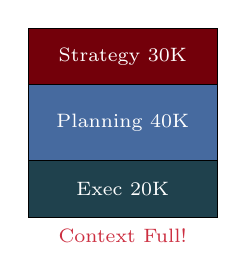
\begin{tikzpicture}[scale=0.8]
                \draw[fill=UofSCSandstorm] (0,0) rectangle (3,3);
                \draw[fill=UofSCGarnet] (0,2.1) rectangle (3,3);
                \draw[fill=UofSCAtlantic] (0,0.9) rectangle (3,2.1);
                \draw[fill=UofSCCongaree] (0,0) rectangle (3,0.9);
                \node[white,font=\scriptsize] at (1.5,2.55) {Strategy 30K};
                \node[white,font=\scriptsize] at (1.5,1.5) {Planning 40K};
                \node[white,font=\scriptsize] at (1.5,0.45) {Exec 20K};
                \node[font=\scriptsize,color=UofSCRose] at (1.5,-0.3) {Context Full!};
            \end{tikzpicture}
            \end{center}
        \end{column}
        \begin{column}{0.5\textwidth}
            \textbf{Three-Layer System:}
            \begin{center}
            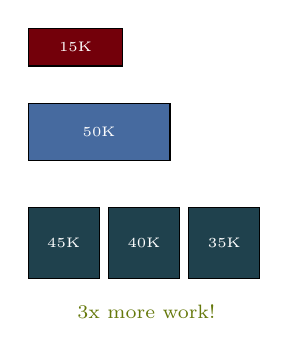
\begin{tikzpicture}[scale=0.6]
                % Strategy box
                \draw[fill=UofSCGarnet] (0,5) rectangle (2,5.8);
                \node[white,font=\tiny] at (1,5.4) {15K};

                % Planning box
                \draw[fill=UofSCAtlantic] (0,3) rectangle (3,4.2);
                \node[white,font=\tiny] at (1.5,3.6) {50K};

                % Execution boxes
                \draw[fill=UofSCCongaree] (0,0.5) rectangle (1.5,2);
                \draw[fill=UofSCCongaree] (1.7,0.5) rectangle (3.2,2);
                \draw[fill=UofSCCongaree] (3.4,0.5) rectangle (4.9,2);
                \node[white,font=\tiny] at (0.75,1.25) {45K};
                \node[white,font=\tiny] at (2.45,1.25) {40K};
                \node[white,font=\tiny] at (4.15,1.25) {35K};

                \node[font=\scriptsize,color=UofSCHorseshoe] at (2.5,-0.2) {3x more work!};
            \end{tikzpicture}
            \end{center}
        \end{column}
    \end{columns}

    \vspace{0.3cm}
    \begin{block}{Context Optimization Techniques}
        \begin{itemize}
            \item Progressive summarization upward
            \item Selective context passing downward
            \item File references instead of full contents
            \item Example-based learning instead of full docs
        \end{itemize}
    \end{block}
\end{frame}

\begin{frame}{Complete Three-Tier Architecture}
    \begin{center}
    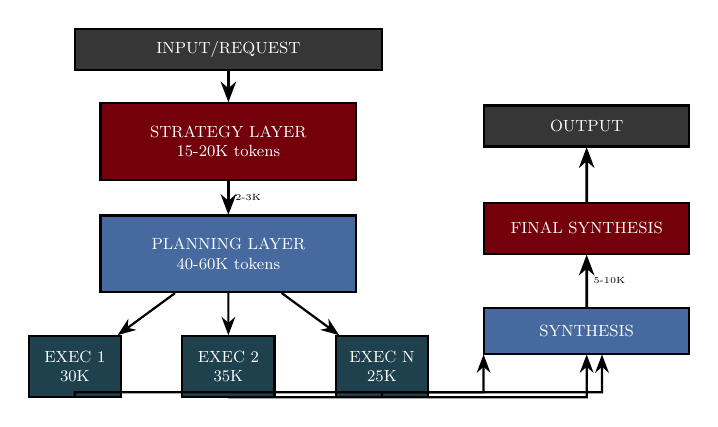
\begin{tikzpicture}[scale=0.65, transform shape]
        % Input
        \node[genericbox, fill=UofSC90Black, text=white, minimum width=6cm] (input) at (0,7) {INPUT/REQUEST};

        % Strategy
        \node[strategynode, minimum width=5cm, minimum height=1.5cm] (strat) at (0,5.2) {STRATEGY LAYER\\15-20K tokens};

        % Planning
        \node[planningnode, minimum width=5cm, minimum height=1.5cm] (plan) at (0,3) {PLANNING LAYER\\40-60K tokens};

        % Execution agents
        \node[execnode, minimum width=1.8cm, minimum height=1.2cm] (exec1) at (-3,0.8) {EXEC 1\\30K};
        \node[execnode, minimum width=1.8cm, minimum height=1.2cm] (exec2) at (0,0.8) {EXEC 2\\35K};
        \node[execnode, minimum width=1.8cm, minimum height=1.2cm] (exec3) at (3,0.8) {EXEC N\\25K};

        % Synthesis
        \node[planningnode, minimum width=4cm] (synth) at (7,1.5) {SYNTHESIS};
        \node[strategynode, minimum width=4cm] (final) at (7,3.5) {FINAL SYNTHESIS};

        % Output
        \node[genericbox, fill=UofSC90Black, text=white, minimum width=4cm] (output) at (7,5.5) {OUTPUT};

        % Arrows
        \draw[myarrow, line width=1pt] (input) -- (strat);
        \draw[myarrow, line width=1pt] (strat) -- node[right,font=\tiny]{2-3K} (plan);
        \draw[myarrow] (plan) -- (exec1);
        \draw[myarrow] (plan) -- (exec2);
        \draw[myarrow] (plan) -- (exec3);

        \draw[myarrow] (exec1) -- ++(0,-0.5) -| (synth.south west);
        \draw[myarrow] (exec2) -- ++(0,-0.6) -| (synth.south);
        \draw[myarrow] (exec3) -- ++(0,-0.5) -| ($(synth.south)+(0.3,0)$);

        \draw[myarrow, line width=1pt] (synth) -- node[right,font=\tiny]{5-10K} (final);
        \draw[myarrow, line width=1pt] (final) -- (output);
    \end{tikzpicture}
    \end{center}

    \textbf{Key Observation:} Execution agents run in parallel. Total time = Strategy + Planning + max(Exec times) + Synthesis, NOT sum of all exec times.
\end{frame}

% ============================================
% SECTION 3: Hierarchical Multi-Agent Systems
% ============================================
\section{Hierarchical Multi-Agent Systems (HMAS)}

\begin{frame}{Introduction to HMAS}
    \begin{columns}[T]
        \begin{column}{0.5\textwidth}
            \textbf{Simple Three-Tier:}
            \begin{center}
            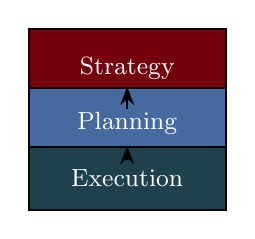
\begin{tikzpicture}[scale=0.7]
                \node[strategynode,minimum width=2.5cm] (s) at (0,3) {Strategy};
                \node[planningnode,minimum width=2.5cm] (p) at (0,2) {Planning};
                \node[execnode,minimum width=2.5cm] (e) at (0,1) {Execution};
                \draw[myarrow] (s) -- (p);
                \draw[myarrow] (p) -- (e);
            \end{tikzpicture}
            \end{center}
        \end{column}
        \begin{column}{0.5\textwidth}
            \textbf{Hierarchical Multi-Agent:}
            \begin{center}
            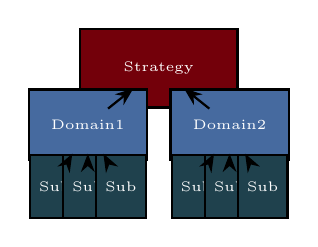
\begin{tikzpicture}[scale=0.6]
                \node[strategynode,minimum width=2cm,font=\tiny] (s) at (0,4) {Strategy};
                \node[planningnode,minimum width=1.5cm,font=\tiny] (d1) at (-1.5,2.8) {Domain1};
                \node[planningnode,minimum width=1.5cm,font=\tiny] (d2) at (1.5,2.8) {Domain2};
                \node[execnode,minimum width=0.6cm,font=\tiny] (e1) at (-2.2,1.5) {Sub};
                \node[execnode,minimum width=0.6cm,font=\tiny] (e2) at (-1.5,1.5) {Sub};
                \node[execnode,minimum width=0.6cm,font=\tiny] (e3) at (-0.8,1.5) {Sub};
                \node[execnode,minimum width=0.6cm,font=\tiny] (e4) at (0.8,1.5) {Sub};
                \node[execnode,minimum width=0.6cm,font=\tiny] (e5) at (1.5,1.5) {Sub};
                \node[execnode,minimum width=0.6cm,font=\tiny] (e6) at (2.2,1.5) {Sub};

                \draw[myarrow] (s) -- (d1);
                \draw[myarrow] (s) -- (d2);
                \draw[myarrow] (d1) -- (e1);
                \draw[myarrow] (d1) -- (e2);
                \draw[myarrow] (d1) -- (e3);
                \draw[myarrow] (d2) -- (e4);
                \draw[myarrow] (d2) -- (e5);
                \draw[myarrow] (d2) -- (e6);
            \end{tikzpicture}
            \end{center}
        \end{column}
    \end{columns}

    \vspace{0.3cm}
    \textbf{HMAS Characteristics:}
    \begin{itemize}
        \item Tree or graph structure of agents
        \item Each parent agent coordinates children
        \item Specialization at each level
        \item Can be arbitrarily deep
        \item Suitable for very complex problems
    \end{itemize}

    \begin{block}{HMAS Enables}
        Specialization at each level, Domain-specific agents, Clear reporting structure, Scalable to large problems, Adaptive restructuring
    \end{block}
\end{frame}

\begin{frame}{Hierarchical Agent Tree Design}
    \begin{center}
    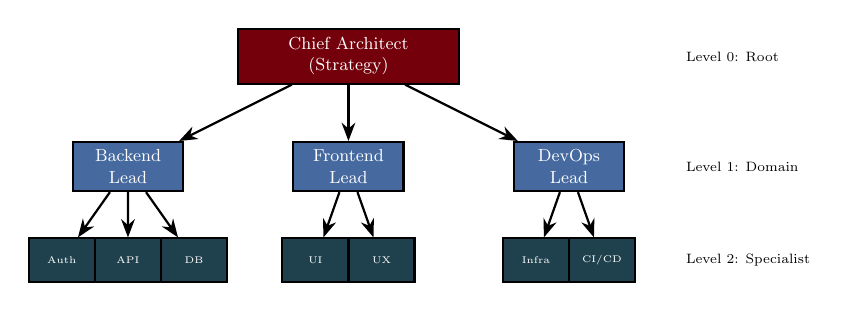
\begin{tikzpicture}[scale=0.7, transform shape]
        % Root
        \node[strategynode, minimum width=4cm] (root) at (0,5.5) {Chief Architect\\(Strategy)};

        % Level 1
        \node[planningnode, minimum width=2cm] (be) at (-4,3.5) {Backend\\Lead};
        \node[planningnode, minimum width=2cm] (fe) at (0,3.5) {Frontend\\Lead};
        \node[planningnode, minimum width=2cm] (ops) at (4,3.5) {DevOps\\Lead};

        % Level 2 - Backend
        \node[execnode, minimum width=1.2cm, font=\tiny] (auth) at (-5.2,1.8) {Auth};
        \node[execnode, minimum width=1.2cm, font=\tiny] (api) at (-4,1.8) {API};
        \node[execnode, minimum width=1.2cm, font=\tiny] (db) at (-2.8,1.8) {DB};

        % Level 2 - Frontend
        \node[execnode, minimum width=1.2cm, font=\tiny] (ui) at (-0.6,1.8) {UI};
        \node[execnode, minimum width=1.2cm, font=\tiny] (ux) at (0.6,1.8) {UX};

        % Level 2 - DevOps
        \node[execnode, minimum width=1.2cm, font=\tiny] (infra) at (3.4,1.8) {Infra};
        \node[execnode, minimum width=1.2cm, font=\tiny] (ci) at (4.6,1.8) {CI/CD};

        % Arrows
        \draw[myarrow] (root) -- (be);
        \draw[myarrow] (root) -- (fe);
        \draw[myarrow] (root) -- (ops);

        \draw[myarrow] (be) -- (auth);
        \draw[myarrow] (be) -- (api);
        \draw[myarrow] (be) -- (db);

        \draw[myarrow] (fe) -- (ui);
        \draw[myarrow] (fe) -- (ux);

        \draw[myarrow] (ops) -- (infra);
        \draw[myarrow] (ops) -- (ci);

        % Level labels
        \node[font=\scriptsize, right] at (6,5.5) {Level 0: Root};
        \node[font=\scriptsize, right] at (6,3.5) {Level 1: Domain};
        \node[font=\scriptsize, right] at (6,1.8) {Level 2: Specialist};
    \end{tikzpicture}
    \end{center}

    \vspace{0.2cm}
    \begin{columns}[T]
        \begin{column}{0.5\textwidth}
            \textbf{Tree Characteristics:}
            \begin{itemize}
                \item Narrow (2-3 children): Deep, specialized
                \item Wide (5-10 children): Flat, general
                \item Balanced (3-5): Recommended
            \end{itemize}
        \end{column}
        \begin{column}{0.5\textwidth}
            \textbf{Parallelization:}
            \begin{itemize}
                \item All siblings run in parallel
                \item Each level multiplies parallelism
                \item Total speedup: product of sibling counts
            \end{itemize}
        \end{column}
    \end{columns}
\end{frame}

\begin{frame}{Leader-Worker Pattern}
    \begin{columns}[T]
        \begin{column}{0.55\textwidth}
            \begin{center}
            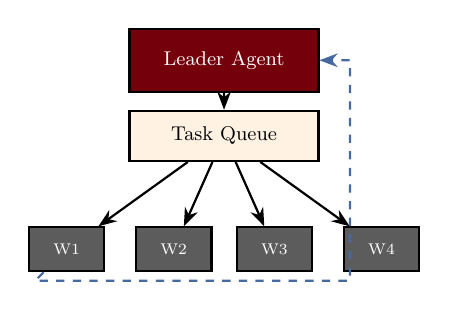
\begin{tikzpicture}[scale=0.8, transform shape]
                % Leader
                \node[leadernode] (leader) at (0,3) {Leader Agent};

                % Task queue
                \node[genericbox, minimum width=3cm, fill=UofSCSandstorm] (queue) at (0,1.8) {Task Queue};

                % Workers
                \node[workernode] (w1) at (-2.5,0) {W1};
                \node[workernode] (w2) at (-0.8,0) {W2};
                \node[workernode] (w3) at (0.8,0) {W3};
                \node[workernode] (w4) at (2.5,0) {W4};

                % Arrows
                \draw[myarrow] (leader) -- (queue);
                \draw[myarrow] (queue) -- (w1);
                \draw[myarrow] (queue) -- (w2);
                \draw[myarrow] (queue) -- (w3);
                \draw[myarrow] (queue) -- (w4);

                % Return arrows
                \draw[myarrow, dashed, color=UofSCAtlantic] (w1) -- ++(-0.5,-0.5) -- ++(5,0) -- ++(0,3.5) -- (leader);
            \end{tikzpicture}
            \end{center}

            \vspace{0.2cm}
            \textbf{Leader Responsibilities:}
            \begin{enumerate}
                \item Task Distribution
                \item Monitoring Progress
                \item Result Aggregation
                \item Error Recovery
            \end{enumerate}
        \end{column}
        \begin{column}{0.45\textwidth}
            \textbf{Load Balancing Strategies:}
            \begin{itemize}
                \item \textbf{Round-Robin:} Simple, fair
                \item \textbf{Work Queue:} FIFO, adaptive
                \item \textbf{Priority Queue:} Optimizes latency
                \item \textbf{Capacity-Based:} Balanced utilization
            \end{itemize}

            \vspace{0.3cm}
            \textbf{Worker Pool Management:}
            \begin{itemize}
                \item Dynamic sizing (scale with load)
                \item Fixed sizing (predictable)
                \item Hybrid (core + temporary)
            \end{itemize}
        \end{column}
    \end{columns}
\end{frame}

\begin{frame}{Domain-Specialized Sub-Agents}
    \begin{columns}[T]
        \begin{column}{0.5\textwidth}
            \begin{center}
            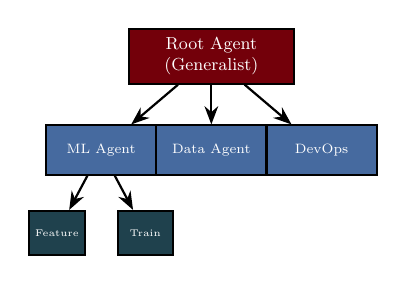
\begin{tikzpicture}[scale=0.7, transform shape]
                \node[strategynode, minimum width=3cm] (root) at (0,4) {Root Agent\\(Generalist)};

                \node[planningnode, minimum width=2cm, font=\scriptsize] (ml) at (-2,2.3) {ML Agent};
                \node[planningnode, minimum width=2cm, font=\scriptsize] (data) at (0,2.3) {Data Agent};
                \node[planningnode, minimum width=2cm, font=\scriptsize] (devops) at (2,2.3) {DevOps};

                \node[execnode, minimum width=1cm, font=\tiny] (fe) at (-2.8,0.8) {Feature};
                \node[execnode, minimum width=1cm, font=\tiny] (train) at (-1.2,0.8) {Train};

                \draw[myarrow] (root) -- (ml);
                \draw[myarrow] (root) -- (data);
                \draw[myarrow] (root) -- (devops);
                \draw[myarrow] (ml) -- (fe);
                \draw[myarrow] (ml) -- (train);
            \end{tikzpicture}
            \end{center}
        \end{column}
        \begin{column}{0.5\textwidth}
            \textbf{Benefits of Specialization:}
            \begin{enumerate}
                \item \textbf{Domain Expertise:} Better decisions
                \item \textbf{Reduced Context:} Better token efficiency
                \item \textbf{Reusability:} Library of experts
                \item \textbf{Parallel Development:} No blocking
            \end{enumerate}
        \end{column}
    \end{columns}

    \vspace{0.3cm}
    \begin{exampleblock}{Specialization Patterns}
        \begin{itemize}
            \item \textbf{Domain Specialists:} ML, Dev, Ops (distinct areas)
            \item \textbf{Task-Phase Specialists:} Design, Code, Test (workflow phases)
            \item \textbf{Technology Specialists:} Backend, Frontend, Database (tech stack)
            \item \textbf{Hybrid:} Mix of domain and phase specialists
        \end{itemize}
    \end{exampleblock}
\end{frame}

% ============================================
% SECTION 4: Agents Calling Agents
% ============================================
\section{Agents Calling Agents}

\begin{frame}{Hierarchical Delegation Patterns}
    \begin{columns}[T]
        \begin{column}{0.55\textwidth}
            \textbf{Fundamental Pattern:}
            \begin{center}
            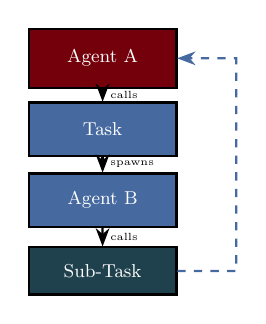
\begin{tikzpicture}[scale=0.75, transform shape]
                \node[strategynode, minimum width=2.5cm] (a) at (0,4) {Agent A};
                \node[planningnode, minimum width=2.5cm] (task) at (0,2.8) {Task};
                \node[planningnode, minimum width=2.5cm] (b) at (0,1.6) {Agent B};
                \node[execnode, minimum width=2.5cm] (subtask) at (0,0.4) {Sub-Task};

                \draw[myarrow] (a) -- node[right,font=\tiny]{calls} (task);
                \draw[myarrow] (task) -- node[right,font=\tiny]{spawns} (b);
                \draw[myarrow] (b) -- node[right,font=\tiny]{calls} (subtask);

                \draw[myarrow, dashed, color=UofSCAtlantic] (subtask.east) -- ++(1,0) -- ++(0,3.6) -- (a.east);
            \end{tikzpicture}
            \end{center}
        \end{column}
        \begin{column}{0.45\textwidth}
            \textbf{Key Difference:}
            \begin{itemize}
                \item Before: Main agent calls tasks (passive)
                \item Now: Tasks can spawn agents
                \item Enables: Recursive delegation
            \end{itemize}

            \vspace{0.3cm}
            \textbf{Benefits:}
            \begin{enumerate}
                \item Delegation to specialists
                \item Specialization at each level
                \item Scalability (recursive decomposition)
                \item Reusability of agent components
            \end{enumerate}
        \end{column}
    \end{columns}

    \vspace{0.2cm}
    \begin{alertblock}{Orchestration Models}
        Hierarchical Delegation, Delegation with Collaboration, Recursive Decomposition, Dynamic Delegation (runtime decisions)
    \end{alertblock}
\end{frame}

\begin{frame}{Context Inheritance Flow}
    \begin{center}
    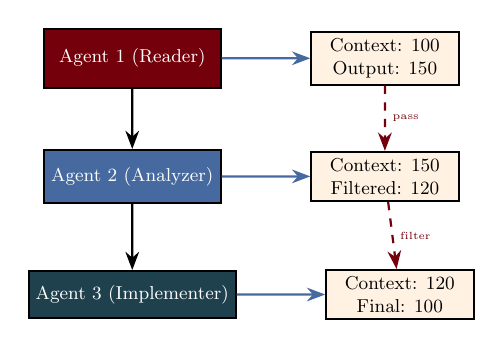
\begin{tikzpicture}[scale=0.75, transform shape]
        % Agents
        \node[strategynode, minimum width=3cm] (a1) at (0,5) {Agent 1 (Reader)};
        \node[planningnode, minimum width=3cm] (a2) at (0,3) {Agent 2 (Analyzer)};
        \node[execnode, minimum width=3cm] (a3) at (0,1) {Agent 3 (Implementer)};

        % Context boxes
        \node[genericbox, fill=UofSCSandstorm, minimum width=2.5cm, right=1.5cm of a1] (c1) {Context: 100\\Output: 150};
        \node[genericbox, fill=UofSCSandstorm, minimum width=2.5cm, right=1.5cm of a2] (c2) {Context: 150\\Filtered: 120};
        \node[genericbox, fill=UofSCSandstorm, minimum width=2.5cm, right=1.5cm of a3] (c3) {Context: 120\\Final: 100};

        % Arrows
        \draw[myarrow] (a1) -- (a2);
        \draw[myarrow] (a2) -- (a3);

        \draw[myarrow, color=UofSCAtlantic] (a1) -- (c1);
        \draw[myarrow, color=UofSCAtlantic] (a2) -- (c2);
        \draw[myarrow, color=UofSCAtlantic] (a3) -- (c3);

        % Filter arrows
        \draw[myarrow, dashed, color=UofSCGarnet] (c1) -- node[right,font=\tiny]{pass} (c2);
        \draw[myarrow, dashed, color=UofSCGarnet] (c2) -- node[right,font=\tiny]{filter} (c3);
    \end{tikzpicture}
    \end{center}

    \vspace{0.3cm}
    \textbf{Context Inheritance Strategies:}
    \begin{columns}[T]
        \begin{column}{0.33\textwidth}
            \textbf{Chain:}
            Result passes through each step
        \end{column}
        \begin{column}{0.33\textwidth}
            \textbf{Filtered:}
            Only relevant context passes
        \end{column}
        \begin{column}{0.33\textwidth}
            \textbf{Reference-Based:}
            Pointers instead of content
        \end{column}
    \end{columns}
\end{frame}

\begin{frame}{Result Consolidation Patterns}
    \begin{columns}[T]
        \begin{column}{0.5\textwidth}
            \textbf{Sequential Consolidation:}
            \begin{center}
            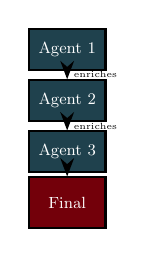
\begin{tikzpicture}[scale=0.65, transform shape]
                \node[execnode, minimum width=1.5cm] (a1) at (0,3) {Agent 1};
                \node[execnode, minimum width=1.5cm] (a2) at (0,2) {Agent 2};
                \node[execnode, minimum width=1.5cm] (a3) at (0,1) {Agent 3};
                \node[strategynode, minimum width=1.5cm] (final) at (0,0) {Final};

                \draw[myarrow] (a1) -- node[right,font=\tiny]{enriches} (a2);
                \draw[myarrow] (a2) -- node[right,font=\tiny]{enriches} (a3);
                \draw[myarrow] (a3) -- (final);
            \end{tikzpicture}
            \end{center}

            \vspace{0.3cm}
            \textbf{Parallel Consolidation:}
            \begin{center}
            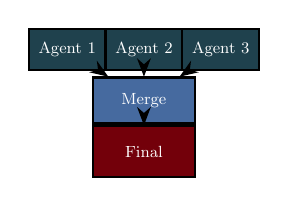
\begin{tikzpicture}[scale=0.65, transform shape]
                \node[execnode, minimum width=1.5cm] (a1) at (-1.5,2) {Agent 1};
                \node[execnode, minimum width=1.5cm] (a2) at (0,2) {Agent 2};
                \node[execnode, minimum width=1.5cm] (a3) at (1.5,2) {Agent 3};
                \node[planningnode, minimum width=2cm] (merge) at (0,1) {Merge};
                \node[strategynode, minimum width=2cm] (final) at (0,0) {Final};

                \draw[myarrow] (a1) -- (merge);
                \draw[myarrow] (a2) -- (merge);
                \draw[myarrow] (a3) -- (merge);
                \draw[myarrow] (merge) -- (final);
            \end{tikzpicture}
            \end{center}
        \end{column}
        \begin{column}{0.5\textwidth}
            \textbf{Merge Strategies:}
            \begin{itemize}
                \item \textbf{Concatenate:} A + B + C
                \item \textbf{Deduplicate:} Remove duplicates
                \item \textbf{Verify:} Check contradictions
                \item \textbf{Synthesize:} Create unified view
            \end{itemize}

            \vspace{0.3cm}
            \textbf{Conflict Resolution:}
            \begin{enumerate}
                \item Priority-Based (architecture wins)
                \item Vote-Based (majority wins)
                \item Consequence-Based (evaluate impact)
                \item Escalation (return to main)
            \end{enumerate}
        \end{column}
    \end{columns}
\end{frame}

\begin{frame}{Limitations of Nested Agent Calls}
    \begin{alertblock}{Key Limitation: Claude Code Cannot Use Nested Subagents}
        Tasks cannot spawn SubAgents from within tasks. All agents must be called from the main agent level.
    \end{alertblock}

    \vspace{0.2cm}
    \textbf{Why This Limitation Exists:}
    \begin{columns}[T]
        \begin{column}{0.5\textwidth}
            \begin{itemize}
                \item \textbf{Token Budget:} Nested calls multiply usage
                \item \textbf{Context Contamination:} Grows exponentially
            \end{itemize}
        \end{column}
        \begin{column}{0.5\textwidth}
            \begin{itemize}
                \item \textbf{Latency:} Each level adds overhead
                \item \textbf{Complexity:} Error handling becomes difficult
            \end{itemize}
        \end{column}
    \end{columns}

    \vspace{0.3cm}
    \textbf{Theoretical Depth Limits:}
    \begin{center}
    \begin{tabular}{lcc}
        \toprule
        \textbf{Depth} & \textbf{Token Usage} & \textbf{Status} \\
        \midrule
        Depth 1 & 27K tokens & OK \\
        Depth 2 & 64K tokens & OK \\
        Depth 3 & 111K tokens & OK \\
        Depth 4 & 168K tokens & OK \\
        Depth 5 & 235K tokens & OVERFLOW \\
        \bottomrule
    \end{tabular}
    \end{center}
    \textit{Practical limit: 3-4 levels of nesting}
\end{frame}

\begin{frame}{Workaround Patterns}
    \begin{columns}[T]
        \begin{column}{0.5\textwidth}
            \textbf{Pattern 1: Flat Delegation}
            \begin{center}
            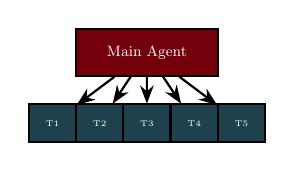
\begin{tikzpicture}[scale=0.6, transform shape]
                \node[strategynode, minimum width=3cm] (main) at (0,2.5) {Main Agent};
                \node[execnode, minimum width=1cm, font=\tiny] (t1) at (-2,1) {T1};
                \node[execnode, minimum width=1cm, font=\tiny] (t2) at (-1,1) {T2};
                \node[execnode, minimum width=1cm, font=\tiny] (t3) at (0,1) {T3};
                \node[execnode, minimum width=1cm, font=\tiny] (t4) at (1,1) {T4};
                \node[execnode, minimum width=1cm, font=\tiny] (t5) at (2,1) {T5};

                \draw[myarrow] (main) -- (t1);
                \draw[myarrow] (main) -- (t2);
                \draw[myarrow] (main) -- (t3);
                \draw[myarrow] (main) -- (t4);
                \draw[myarrow] (main) -- (t5);
            \end{tikzpicture}
            \end{center}
            All coordination at main level

            \vspace{0.3cm}
            \textbf{Pattern 2: Role-Based Shared State}
            \begin{itemize}
                \item Shared context between agents
                \item Reader $\rightarrow$ Planner $\rightarrow$ Coder $\rightarrow$ Tester
            \end{itemize}
        \end{column}
        \begin{column}{0.5\textwidth}
            \textbf{Pattern 3: Hierarchical Tasks}
            \begin{itemize}
                \item Subtasks with own context
                \item Simulates deeper nesting
            \end{itemize}

            \vspace{0.3cm}
            \textbf{Pattern 4: Pipeline with Files}
            \begin{itemize}
                \item Agent 1 $\rightarrow$ File 1 $\rightarrow$ Agent 2
                \item Coordination through artifacts
            \end{itemize}

            \vspace{0.3cm}
            \textbf{Pattern 5: Domain Specialists}
            \begin{itemize}
                \item Different main agents per domain
                \item Root orchestrator coordinates
            \end{itemize}
        \end{column}
    \end{columns}

    \vspace{0.3cm}
    \begin{block}{Recommendation}
        Claude Code uses Pattern 1 (Flat Delegation). Most problems can be solved with 3-5 parallel execution agents coordinated from main.
    \end{block}
\end{frame}

% ============================================
% SECTION 5: Five-Phase Workflow
% ============================================
\section{Five-Phase Workflow}

\begin{frame}{The Five-Phase Model}
    \begin{center}
    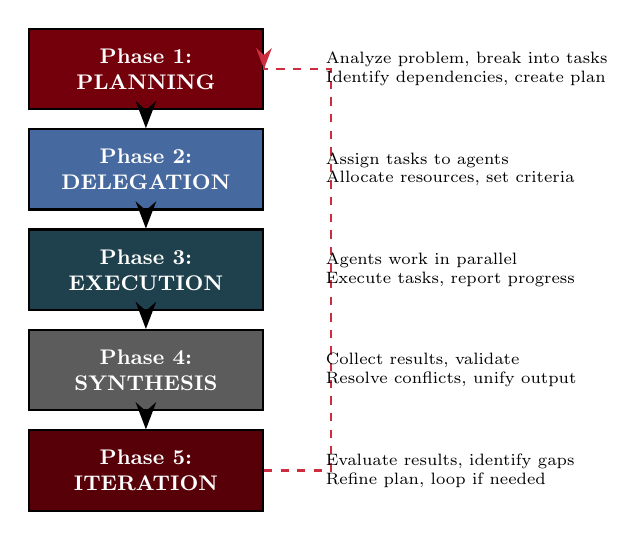
\begin{tikzpicture}[scale=0.85, transform shape]
        % Phase boxes
        \node[phasebox, fill=UofSCGarnet, text=white] (p1) at (0,5) {Phase 1:\\PLANNING};
        \node[phasebox, fill=UofSCAtlantic, text=white] (p2) at (0,3.5) {Phase 2:\\DELEGATION};
        \node[phasebox, fill=UofSCCongaree, text=white] (p3) at (0,2) {Phase 3:\\EXECUTION};
        \node[phasebox, fill=UofSC70Black, text=white] (p4) at (0,0.5) {Phase 4:\\SYNTHESIS};
        \node[phasebox, fill=UofSCDarkGarnet, text=white] (p5) at (0,-1) {Phase 5:\\ITERATION};

        % Arrows
        \draw[myarrow, line width=1.5pt] (p1) -- (p2);
        \draw[myarrow, line width=1.5pt] (p2) -- (p3);
        \draw[myarrow, line width=1.5pt] (p3) -- (p4);
        \draw[myarrow, line width=1.5pt] (p4) -- (p5);

        % Feedback loop
        \draw[myarrow, line width=1pt, dashed, color=UofSCRose] (p5.east) -- ++(1,0) -- ++(0,6) -- ++(-1,0) -- (p1.east);

        % Descriptions
        \node[font=\scriptsize, align=left, right=0.8cm of p1] {Analyze problem, break into tasks\\Identify dependencies, create plan};
        \node[font=\scriptsize, align=left, right=0.8cm of p2] {Assign tasks to agents\\Allocate resources, set criteria};
        \node[font=\scriptsize, align=left, right=0.8cm of p3] {Agents work in parallel\\Execute tasks, report progress};
        \node[font=\scriptsize, align=left, right=0.8cm of p4] {Collect results, validate\\Resolve conflicts, unify output};
        \node[font=\scriptsize, align=left, right=0.8cm of p5] {Evaluate results, identify gaps\\Refine plan, loop if needed};
    \end{tikzpicture}
    \end{center}
\end{frame}

\begin{frame}{Five-Phase Workflow Details}
    \begin{columns}[T]
        \begin{column}{0.5\textwidth}
            \textbf{Phase 1: PLANNING}
            \begin{itemize}
                \item Parse request
                \item Understand domain
                \item Identify major phases
                \item Analyze dependencies
                \item Estimate resources
            \end{itemize}

            \vspace{0.2cm}
            \textbf{Phase 2: DELEGATION}
            \begin{itemize}
                \item Categorize tasks
                \item Select appropriate agents
                \item Prepare context for each
                \item Determine parallelization
            \end{itemize}
        \end{column}
        \begin{column}{0.5\textwidth}
            \textbf{Phase 3: EXECUTION}
            \begin{itemize}
                \item Spawn agents
                \item Execute tasks
                \item Handle local errors
                \item Collect results
            \end{itemize}

            \vspace{0.2cm}
            \textbf{Phase 4: SYNTHESIS}
            \begin{itemize}
                \item Check completeness
                \item Validate consistency
                \item Integrate outputs
                \item Generate report
            \end{itemize}

            \vspace{0.2cm}
            \textbf{Phase 5: ITERATION}
            \begin{itemize}
                \item Evaluate against criteria
                \item Identify gaps
                \item Loop if needed
            \end{itemize}
        \end{column}
    \end{columns}
\end{frame}

\begin{frame}{Agent Delegation Patterns}
    \begin{center}
    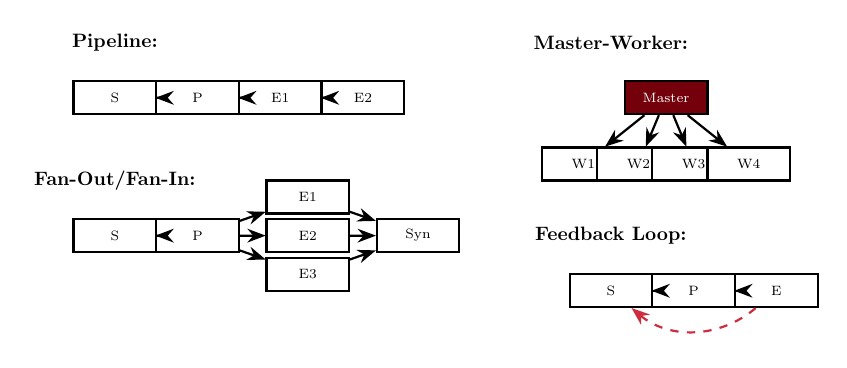
\begin{tikzpicture}[scale=0.7, transform shape]
        % Pattern 1: Pipeline
        \node[font=\bfseries] at (-4,5) {Pipeline:};
        \node[smallbox] (pa1) at (-4,4) {S};
        \node[smallbox] (pa2) at (-2.5,4) {P};
        \node[smallbox] (pa3) at (-1,4) {E1};
        \node[smallbox] (pa4) at (0.5,4) {E2};
        \draw[myarrow] (pa1) -- (pa2);
        \draw[myarrow] (pa2) -- (pa3);
        \draw[myarrow] (pa3) -- (pa4);

        % Pattern 2: Fan-Out/Fan-In
        \node[font=\bfseries] at (-4,2.5) {Fan-Out/Fan-In:};
        \node[smallbox] (fb1) at (-4,1.5) {S};
        \node[smallbox] (fb2) at (-2.5,1.5) {P};
        \node[smallbox] (fb3) at (-0.5,2.2) {E1};
        \node[smallbox] (fb4) at (-0.5,1.5) {E2};
        \node[smallbox] (fb5) at (-0.5,0.8) {E3};
        \node[smallbox] (fb6) at (1.5,1.5) {Syn};
        \draw[myarrow] (fb1) -- (fb2);
        \draw[myarrow] (fb2) -- (fb3);
        \draw[myarrow] (fb2) -- (fb4);
        \draw[myarrow] (fb2) -- (fb5);
        \draw[myarrow] (fb3) -- (fb6);
        \draw[myarrow] (fb4) -- (fb6);
        \draw[myarrow] (fb5) -- (fb6);

        % Pattern 3: Master-Worker
        \node[font=\bfseries] at (5,5) {Master-Worker:};
        \node[smallbox, fill=UofSCGarnet, text=white] (mw1) at (6,4) {Master};
        \node[smallbox] (mw2) at (4.5,2.8) {W1};
        \node[smallbox] (mw3) at (5.5,2.8) {W2};
        \node[smallbox] (mw4) at (6.5,2.8) {W3};
        \node[smallbox] (mw5) at (7.5,2.8) {W4};
        \draw[myarrow] (mw1) -- (mw2);
        \draw[myarrow] (mw1) -- (mw3);
        \draw[myarrow] (mw1) -- (mw4);
        \draw[myarrow] (mw1) -- (mw5);

        % Pattern 4: Feedback Loop
        \node[font=\bfseries] at (5,1.5) {Feedback Loop:};
        \node[smallbox] (fl1) at (5,0.5) {S};
        \node[smallbox] (fl2) at (6.5,0.5) {P};
        \node[smallbox] (fl3) at (8,0.5) {E};
        \draw[myarrow] (fl1) -- (fl2);
        \draw[myarrow] (fl2) -- (fl3);
        \draw[myarrow, dashed, color=UofSCRose] (fl3) to[bend left=40] (fl1);
    \end{tikzpicture}
    \end{center}

    \vspace{0.3cm}
    \begin{block}{Pattern Selection Guide}
        \textbf{Pipeline:} Strict ordering | \textbf{Fan-Out:} Parallel then consolidate | \textbf{Master-Worker:} Many similar tasks | \textbf{Feedback:} Iterative refinement
    \end{block}
\end{frame}

% ============================================
% SECTION 6: Best Practices
% ============================================
\section{Best Practices}

\begin{frame}{Best Practices for Multi-Tier Systems}
    \begin{columns}[T]
        \begin{column}{0.5\textwidth}
            \textbf{1. Clear Layer Boundaries}
            \begin{itemize}
                \item[\checkmark] Each layer has specific responsibilities
                \item[\checkmark] Information flows through defined interfaces
                \item[$\times$] Strategy layer executing code
            \end{itemize}

            \vspace{0.2cm}
            \textbf{2. Explicit Success Criteria}
            \begin{itemize}
                \item[\checkmark] Define how layer knows when done
                \item[\checkmark] Each layer validates its work
                \item[$\times$] Ambiguous success definitions
            \end{itemize}

            \vspace{0.2cm}
            \textbf{3. Context Management}
            \begin{itemize}
                \item[\checkmark] Sufficient, not excessive, context
                \item[\checkmark] Summarize results upward
                \item[$\times$] Pass 100K tokens to strategy
            \end{itemize}
        \end{column}
        \begin{column}{0.5\textwidth}
            \textbf{4. Error Handling}
            \begin{itemize}
                \item[\checkmark] Explicit error reporting with root cause
                \item[\checkmark] Graceful degradation and fallbacks
                \item[$\times$] Silent failures
            \end{itemize}

            \vspace{0.2cm}
            \textbf{5. Monitoring and Logging}
            \begin{itemize}
                \item[\checkmark] Track execution through all layers
                \item[\checkmark] Log decision points and reasoning
                \item[$\times$] Ignore performance bottlenecks
            \end{itemize}

            \vspace{0.2cm}
            \textbf{6. Testing}
            \begin{itemize}
                \item[\checkmark] Unit test each layer independently
                \item[\checkmark] Integration test layer interactions
                \item[$\times$] Only test individual agents
            \end{itemize}
        \end{column}
    \end{columns}
\end{frame}

\begin{frame}{Failure Modes and Recovery}
    \begin{center}
    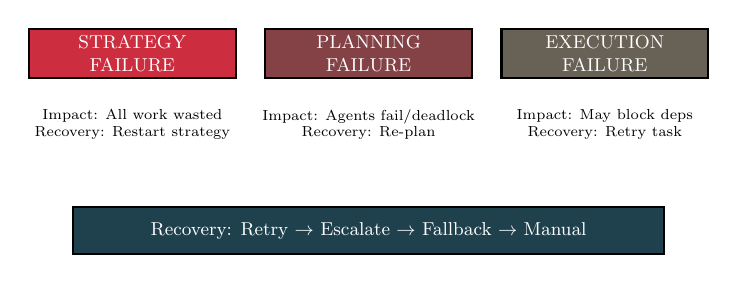
\begin{tikzpicture}[scale=0.75, transform shape]
        % Failure types
        \node[genericbox, fill=UofSCRose, text=white, minimum width=3.5cm] (f1) at (-4,3) {STRATEGY\\FAILURE};
        \node[genericbox, fill=UofSCAzalea, text=white, minimum width=3.5cm] (f2) at (0,3) {PLANNING\\FAILURE};
        \node[genericbox, fill=UofSCWarmGrey, text=white, minimum width=3.5cm] (f3) at (4,3) {EXECUTION\\FAILURE};

        % Impact indicators
        \node[font=\scriptsize, align=center] at (-4,1.8) {Impact: All work wasted\\Recovery: Restart strategy};
        \node[font=\scriptsize, align=center] at (0,1.8) {Impact: Agents fail/deadlock\\Recovery: Re-plan};
        \node[font=\scriptsize, align=center] at (4,1.8) {Impact: May block deps\\Recovery: Retry task};

        % Recovery strategy
        \node[genericbox, fill=UofSCCongaree, text=white, minimum width=10cm] (rec) at (0,0) {Recovery: Retry $\rightarrow$ Escalate $\rightarrow$ Fallback $\rightarrow$ Manual};
    \end{tikzpicture}
    \end{center}

    \vspace{0.3cm}
    \textbf{Recovery Strategies:}
    \begin{columns}[T]
        \begin{column}{0.5\textwidth}
            \begin{itemize}
                \item \textbf{Simple Fallback:} Use prior version
                \item \textbf{Degraded Mode:} Partial solution OK
                \item \textbf{Manual:} Human intervention
            \end{itemize}
        \end{column}
        \begin{column}{0.5\textwidth}
            \begin{itemize}
                \item \textbf{Skip:} Continue without task
                \item \textbf{Compensate:} Alternative approach
                \item \textbf{Circuit Breaker:} Stop retrying
            \end{itemize}
        \end{column}
    \end{columns}
\end{frame}

\begin{frame}{Performance Metrics}
    \begin{columns}[T]
        \begin{column}{0.5\textwidth}
            \textbf{Speed Metrics:}
            \begin{itemize}
                \item Total execution time
                \item Layer breakdown
                \item Parallelization ratio
                \item Coordination overhead
            \end{itemize}

            \vspace{0.3cm}
            \textbf{Efficiency Metrics:}
            \begin{itemize}
                \item Context efficiency (tokens used/available)
                \item Task success rate
                \item Retry rate
                \item Resource utilization
            \end{itemize}
        \end{column}
        \begin{column}{0.5\textwidth}
            \textbf{Quality Metrics:}
            \begin{itemize}
                \item Success criteria met (\%)
                \item Error rate
                \item Result correctness
                \item User satisfaction
            \end{itemize}

            \vspace{0.3cm}
            \textbf{Scalability Metrics:}
            \begin{itemize}
                \item Throughput (tasks/time)
                \item Latency vs. problem size
                \item Resource growth
                \item Agent utilization
            \end{itemize}
        \end{column}
    \end{columns}

    \vspace{0.3cm}
    \begin{exampleblock}{Speedup Example}
        Sequential (2-tier): $1 + 2 + 10 = 13$ seconds\\
        Parallel (3-tier, 3 workers): $1 + 2 + \max(4,3,3) + 1 = 8$ seconds\\
        \textbf{Speedup: 1.63x}
    \end{exampleblock}
\end{frame}

% ============================================
% SUMMARY AND CONCLUSION
% ============================================
\section{Summary}

\begin{frame}{Key Takeaways}
    \begin{columns}[T]
        \begin{column}{0.5\textwidth}
            \textbf{Multi-Tier Architecture:}
            \begin{enumerate}
                \item Three-tier is the practical foundation
                \item Strategy $\rightarrow$ Planning $\rightarrow$ Execution
                \item Parallelization at execution layer
                \item Context management is critical
            \end{enumerate}

            \vspace{0.3cm}
            \textbf{HMAS Principles:}
            \begin{enumerate}
                \item Tree structure with specialists
                \item Leader-worker for parallel work
                \item Domain specialization benefits
                \item Clear coordination protocols
            \end{enumerate}
        \end{column}
        \begin{column}{0.5\textwidth}
            \textbf{Five-Phase Workflow:}
            \begin{enumerate}
                \item Plan $\rightarrow$ Delegate $\rightarrow$ Execute
                \item Synthesize $\rightarrow$ Iterate
                \item Feedback loops for refinement
            \end{enumerate}

            \vspace{0.3cm}
            \textbf{Practical Considerations:}
            \begin{enumerate}
                \item Claude Code: flat multi-agent (3-5)
                \item Token budgets constrain depth
                \item Workaround patterns exist
                \item Design for your constraints
            \end{enumerate}
        \end{column}
    \end{columns}

    \vspace{0.3cm}
    \begin{block}{Core Insight}
        Multi-tier systems add complexity. Use them when: problem naturally decomposes, different expertise needed, parallelization beneficial, and results need intelligent aggregation.
    \end{block}
\end{frame}

\begin{frame}{Questions?}
    \begin{center}
        \vspace{1cm}
        {\Large\textbf{Part 6: Multi-Tier Agent Architecture}}

        \vspace{0.5cm}
        Building Hierarchical Systems with Agentic Coding Tools

        \vspace{1cm}
        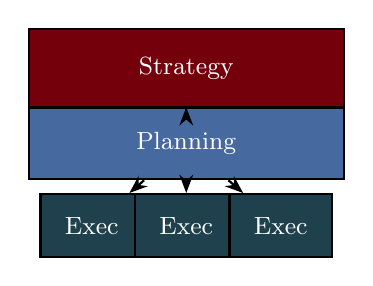
\begin{tikzpicture}[scale=0.8]
            \node[strategynode, minimum width=4cm] (s) at (0,3) {Strategy};
            \node[planningnode, minimum width=4cm] (p) at (0,1.8) {Planning};
            \node[execnode, minimum width=1.3cm] (e1) at (-1.5,0.5) {Exec};
            \node[execnode, minimum width=1.3cm] (e2) at (0,0.5) {Exec};
            \node[execnode, minimum width=1.3cm] (e3) at (1.5,0.5) {Exec};

            \draw[myarrow] (s) -- (p);
            \draw[myarrow] (p) -- (e1);
            \draw[myarrow] (p) -- (e2);
            \draw[myarrow] (p) -- (e3);
        \end{tikzpicture}

        \vspace{1cm}
        \textcolor{UofSCGarnet}{\textbf{University of South Carolina}}
    \end{center}
\end{frame}

\end{document}
